\begin{savequote}[75mm] 
	Good judgment comes from experience, and a lot of that comes from bad judgment.
	\qauthor{Will Rogers} 
\end{savequote}

\chapter{Summarization evaluation}
\label{chap:eval}


Evaluating summarization systems is one of the most difficult tasks. 
It is not clear which is the perfect summary, since humans produce different summaries and yet we can consider them all good. 
Also, the evaluation must be accurate, objective and fast. 
This led to the appearance of many evaluation methods which can be automatic, manual or semi-automatic. 
Many workshops have been organized to evaluate the performance of summarization methods, and test how effective evaluation methods are.

In this chapter we will present some evaluation methods, both intrinsic and extrinsic ones. 
The intrinsic ones seek to evaluate a system in of itself, while the extrinsic ones search to determine the effect of summarization on other tasks.
Then, we will enlist some famous evaluation workshops and campaigns in the context of \ac{ats}. 
Finally, we will discuss these evaluation methods focusing on their advantages and limits.

\section{Evaluation methods}

\ac{ats} evaluation methods can be considered as intrinsic or extrinsic \citep{01-mani}.
Intrinsic evaluation is meant to evaluate the system in of itself. 
It is based on two criteria: summary coherence and summary informativeness. %These criteria are explained later
In the other hand, extrinsic evaluation seeks to determine the effect of summarization on other tasks. 
Figure \ref{fig:eval-classif} represents the different categories of summarization evaluation, as described in \citep{01-mani}.
%
\begin{figure}[!ht]
	\begin{center}
		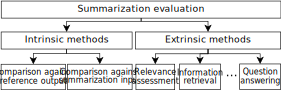
\includegraphics[width=.75\textwidth]{figures/evaluation/eval-classif.pdf} % % %[width=140mm]
		\caption{Classification of evaluation methods.}
		\label{fig:eval-classif}
	\end{center}
\end{figure}

\subsection{Intrinsic evaluation}

The evaluation can be done by comparing the generated summary to the original text or to a reference summary. 
When the system's summary is compared to the original text, actually, we look for the quantity of information recovered; more like information retrieval systems.
Comparing it to a reference summary will allow us to quantify how good the system can be against humans.
%two criteria of evaluation
Also, the intrinsic methods can be seen as: text quality evaluation methods or content evaluation methods \citep{12-steinberger-jezek}.
Text quality evaluation methods attempt to verify linguistic aspects of the generated summary such as grammaticality, reference clarity and coherence. 
The content evaluation methods can be divided into two sub-classes: co-selection methods which evaluate the system based on selecting the right sentences, and content based methods which go deeper by using smaller units such words and n-grams.

% .Recall, Precision, F-score
Given a summarizer which takes an input document $E$ and generates a summary $S$, and given a reference (model) summary $M$ which is some preselected sentences from $ E $; we can define the following relations: 
TP (true positive), TN (true negative), FP (false positive) and FN (false negative).
\begin{itemize}
	\item TP (true positive): the pertinent information captured by $M$ and $S$, so $M \cap S$.
	\item TN (true negative): the pertinent information not captured by $M$ and $S$, so $E - (M \cup S)$.
	\item FP (false positive): the pertinent information captured by $M$ and not captured by $S$, so $M - S$.
	\item FN (false negative): the pertinent information not captured by $M$ and captured by $S$, so $S - M$.
\end{itemize}
The recall is the quantity of right information recovered by a system comparing to what the it should recover (see Equation \ref{eq:recall}).
\begin{equation}
	\label{eq:recall}
	R = \frac {TP} {TP + FN} = \frac {M \cap S} {S}
\end{equation}
%
The precision is the quantity of right information recovered by a system comparing to what it has recovered (see Equation \ref{eq:precision}).
\begin{equation}
	\label{eq:precision}
	P = \frac {TP} {TP + FP} = \frac {M \cap S} {M}
\end{equation}
%
The F-Score is a mix between the recall and the precision using harmonic mean (see Equation \ref{eq:f-score}). 
If $ \beta $ is more than one (1), the recall is advantaged. 
If it is less than one, the precision is advantaged. 
The most used F-Score is F1-score which is a trade-off between recall and precision.
\begin{equation}
	\label{eq:f-score}
	F_{\beta} = \frac
	{(1+\beta^2) P \times R}
	{ \beta^2 P + R}
\end{equation}
We have to say, this type of evaluation does not give systems credit if they choose other sentences similar to the preselected ones. 
It may be useful to use when the summary must contain a precise information from the input text. 
But, in general, to evaluate a summarization system it must be avoided, especially for abstractive methods.

% .ROUGE
\acf{rouge}\footnote{ROUGE: \url{http://www.berouge.com/Pages/default.aspx} [November 23, 2016]}, proposed by \citet{03-Lin-hovy}, is a method inspired from another used for automatic translation evaluation called \ac{bleu} \citep{02-papineni-al}. 
The objective is to automatically measure the quality of the generated summary compared to a reference one.
The idea is to compute the number of units (N-grams) in both system's summary and reference one and calculate the recall.
Since a text can have many summaries, this method allows using many reference summaries.
Many variances of ROUGE have been proposed \citep{04-lin}: ROUGE-N, ROUGE-L, ROUGE-W, ROUGE-S, et ROUGE-SU. 
Equation \ref{eq:rouge-n} describes how ROUGE-N recall is calculated.
\begin{equation}
	\label{eq:rouge-n}
	ROUGE-(N) = \frac{\sum_{S \in Summ_{ref}}{\sum_{N-gram \in S}{Count_{match} (N-gram)}}}
	{\sum_{S \in Summ_{ref}}{\sum_{N-gram \in S}{Count (N-gram)}}}
\end{equation}
Where, \textit{N} is the size of the N-gramme, 
$count_{match}(N-gram)$ is the number of N-grammes found in both candidate and reference summaries. 
$Count (N-gram)$ is the number of N-grammes in the reference summary. 

% .Pyramids
Using similarity measure between automatic summary and human-made one can present some limitations \citep{07-nenkova-al}:
human variation, analyze granularity, semantic equivalence, semantic equivalence and the comparison between extractive and abstractive summaries.
\begin{itemize}
	\item Human variation: different people can select different sentences to incorporate into their summaries. 
	Even the same person can produce two different summaries for the same document.
	
	\item Analyze granularity: even if the system does not choose the same sentence as the model's, it can be pertinent to one sentence or plus in that model.
	
	\item Semantic equivalence: different sentences can express the same thing, even using different words.
	The annotators must choose one sentence out of equivalent sentences, and the system which choose two equivalent sentences must be penalized.
	
	\item Extractive or abstractive? Humans use abstractive summaries; A person use their own words to edit a summary.
	This is why the exact comparison between the reference's and the system's summaries is not possible.
	
\end{itemize}
Pyramid \citep{07-nenkova-al} comes to solve these limitations using a semi-automatic approach. 
Given a number of reference summaries, annotators are asked to define \acp{scu} where the weight of each \ac{scu} can be calculated as the number of relative reference summaries. 
The process of defining the \acp{scu} is not given, they can be as small as modifiers of a noun phrase or as large as a clause. 
The \acp{scu} are regrouped in a pyramid of $ n $ tiers, where $ n $ is the maximum weight of \acp{scu}. 
So an \acp{scu} which belongs to the tier $ T_i $ will have a score of $ i $, where $ |T_i| $ is the number of SCUs in this tier.
For a summary with $ X $ \acp{scu}, Equation \ref{eq:pyramid} shows the optimal content score, where \acp{scu} which do not belong to the pyramid will have a zero weight.
\begin{equation}
	\label{eq:pyramid}
	\max = \sum\limits_{i=j+1}^{n} i * |T_i| + j * (X - \sum\limits_{i=j+1}^{n} |T_i|),
	\text{ where } j = \max\limits_i (\sum\limits_{t = i}^{n} |T_t| \ge X)
\end{equation}

% .BE
\acp{be} are minimal semantic units which can be extracted from a sentence \citep{06-hovy-al}. 
Their goal is to automate summaries evaluation in contrast of Pyramids which needs human involvement. 
This later can introduce some problems such as human variability and evaluation expensiveness in time and cost.
To evaluate a summary, three different modules are proposed: \ac{be} breakers, \ac{be} matchers and \ac{be} scorers. 
The first one is used to break the text into \acp{be} which are defined by \citep{06-hovy-al} as:
``\textit{1- The head of a major syntactic constituent (noun, verb, adjective or adverbial phrases), expressed as a 	single item, or, 2- A relation between a head-BE and a single dependent, expressed as a triple (head | modifier | relation)}".
The matching of \acp{be} is either lexical, using lemmas, using synonyms from Wordnet \citep{95-miller}, using paraphrases or using semantic generalization.
Each BE gets a weight of 1 point for each related reference summary.

% .MeMoG and .AutoSummENG
\ac{autosummeng} \citep{06-giannakopoulos-al} attempts to be language neutral, fully automatic and context sensitive.
The method is based on n-grams, so to be language neutral no preprocessing must be done, this is why the n-grams are extracted over the characters.
Then, a graph is constructed where the n-grams represent its nodes and each arc connecting two n-grams is the number of times these n-grams are judged as neighbors given a distance window $ D_w $. 
Given two summaries $ S_i $ and $ S_j $ with a set of graphs $ \mathbb{G}_1 $ and $ \mathbb{G}_2 $ respectively, and given two graphs $ G^i \in \mathbb{G}_1 $ and $ G^j \in \mathbb{G}_2 $ with the same rank of n-grams, the value similarity is given in Equation~\ref{eq:val-sim}.
\begin{equation}
	\label{eq:val-sim}
	VS(G^i, G^j) = 
	\frac{\sum_{e \in G^i} \left(\mu(e, G^j) * \frac{min(w_e^i, w_e^j)}{min(w_e^i, w_e^j)}\right)}{max(|G^i|, |G^j|)}
\end{equation}
With $ \mu $ as the membership function, which returns 1 when $ e \in G^j $ and 0 otherwise.
$ w_e^i,\ w_e^j $ are the weights of the edges of the element $ e $ in the graphs $ G^i,\ G^j $ respectively.
The overall similarity of $ \mathbb{G}_1 $ and $ \mathbb{G}_2 $ is the weighted sum of the $ VS $ over all ranks (Equation \ref{eq:oval-sim}).
\begin{equation}
	\label{eq:oval-sim}
	VS^O(\mathbb{G}_1, \mathbb{G}_2) = 
	\frac{\sum_{r \in [L_{min}, L_{max}] } r * VS^r }{\sum_{r \in [L_{min}, L_{max}]} r}
\end{equation}
Where $ r $ is the rank of n-grams; 
$ L_{min},\ L_{max} $ are the minimum and the maximum rank of n-grams; 
$ VS^r $ is the value similarity using the graphs with n-gram of rank $ r $.
The grade of a summary is the average of all its similarities with the reference summaries. 
\ac{memog} is somehow a variant of \ac{autosummeng}, where all the graphs of reference summaries are merged into one graph \citep{10-giannakopoulos-karkaletsis}.

% .NPowER.
\ac{npower} \citep{13-giannakopoulos-karkaletsis} is a combination of many of the past metrics via optimization. 
The idea is to create a method which stands as an independent judge to combine the different metrics grades into a better estimate. 
Machine learning (linear regression) is used to estimate the final grade. 
Given a vector of features $ \overline{x} \in \overline{X}  $ (here, \ac{rouge}, \ac{be}, etc.) and a target numeric feature $ y \in \mathbb{R},\ y = f(\overline{x}) $, where $ f $ is an unknown function (human scores or Pyramid scores), the idea is to estimate a combination function $ \tilde{f} $ as shown in Equation \ref{eq:npower}.
\begin{equation}
	\label{eq:npower}
	\tilde{f}: \overline{X} \rightarrow \mathbb{R}: 
	\sum (\tilde{f}(\overline{x}) - f(\overline{x}))^2 \rightarrow 0,\ \forall \overline{x} \in \overline{X}
\end{equation}

Based on the expansiveness of summarization systems evaluated by these past metrics, we can say that these metrics are meant for background systems. 
But, how about update systems? In case we want to evaluate automatic summaries in term of new information which they contain.
Nouveau-ROUGE \citep{11-conroy-al} is a method based on \ac{rouge} metrics to evaluate update summaries. 
The idea is to calculate ROUGE score between an original summary and an update one, then a high \ac{rouge} score indicates high redundancy.
In TREC temporal summarization task \citep{13-aslam-al}, many metrics are proposed to address this issue. 
Given an event (Wikipedia event pages), gold standard updates called nuggets are extracted  and annotated to form a set of nuggets $ \mathcal{N} $ such as a nugget $ n \in \mathcal{N} $ has the properties: the time-stamp of revision history $ n.t $ and the importance provided by assessors (0: no importance to 3: high importance) $ n.i $. 
The evaluation metrics are designed to measure the degree to which a system can generate these nuggets in a timely manner.
Each system must generate a summary $ S $ containing some updates, where an update $ u $ is a sentence length text ($ u.string $) having a time-stamp $ u.t $.
The earliest update $ u $ that match a nugget $ n $ is defined as $ M(n, S) = \text{\textit{argmin}}_{u \in S: u \approx n} u.t $.
Then, the inverse function is defined as $ M^{-1}(u, S) = \{ n \in \mathcal{N}; M(n, S) = u \} $.
The first metric is \textit{Expected Gain metric} (EG) which is similar to traditional notions of precision in IR evaluation (see Equation \ref{eq:eg}). 
When using latency discount, the chosen latency step was $ \alpha = 3600 * 6$ (6 hours).
%
\begin{equation}
	\label{eq:eg}
	%.EG(S) = \frac{1}{|S|} \sum\limits_{\{n \in N: M(n,S) \ne 0 \}} g(M(n,S), n)
	EG(S) = \frac{1}{|S|} \sum\limits_{u \in S} G(u, S)
\end{equation}
Where, 
\[
%G(u, n) = \sum\limits_{n \in M^{-1} (u, \mathcal{S})} g(u, n)
G(u, n) = \sum\limits_{n \in M^{-1} (u, S)} R(n) * \text{\textit{discounting factor}}
\]
%\[
%g(u, n) = R(n) * \text{\textit{discounting factor}}
%\]
\[
R(n) = \left\lbrace\begin{tabular}{ll}
Graded:& $ \frac{e^{n.i}}{e^{\max_{n' \in \mathcal{N}} n'.i}} $ \\
Binary:& $ 1 $ if  ($ n.i > 0 $), $ 0 $ otherwise
\end{tabular}\right.
\]
\[
\textit{discounting factor} = \left\lbrace\begin{tabular}{l}
Discount-free gain: $ 1 $ \\
Latency-discounted gain: $ L(n.t, u.t) = 1 - \frac{2}{\pi} \arctan(\frac{u.t - n.t}{\alpha}) $ 
\end{tabular}\right. 
\]
%
Another metric is \textit{Comprehensiveness metric} C(S) which is similar to traditional notions of recall in IR evaluation (see Equation \ref{eq:cs}).
\begin{equation}
	\label{eq:cs}
	C(S) = \frac{1}{\sum_{n \in \mathcal{N}} R(n)} \sum\limits_{u \in S} G(u, S)
\end{equation}


\subsection{Extrinsic evaluation}

\ac{ats} is, often, used to complete other tasks like executing instructions, information retrieval, question answering, relevance assessment, etc. 
To evaluate how well a summarization system is doing leads to evaluate its effectiveness towards its related task. 
In the relevance assessment task, the assessors try to score how well a summary is related to a given subject.
Another example is reading comprehension task where a human judge is asked to answer some questions based on the original document, then on its summary.
The correct answers number is considered as the score of this summary.

%. SUMMAC extrinsic task
In TIPSTER SUMMAC evaluation \citep{99-mani-al}, two tasks are proposed to evaluate the impact of \ac{ats} on real world tasks: ad-hoc task and categorization task. 
In ad-hoc task, the purpose is to test the pertinence of indicative summaries towards a particular topic.
Given a document (summary or source text), a human subject is asked to determine its relevance to a given topic description, ignoring whether it was a full text or a summary.
The accuracy of the subjects is measured on how well they can indicate the relevance between the subjects and their relative full texts. 
Then the recall, precision and F1-score are calculated for the participants systems. 
In categorization task, the purpose is to determine if a generic summary contains enough information to allow an analyst categorizing a document as quickly and correctly as possible. 
The evaluation is proceeded as in ad-hoc task's.
But after reading the document, the human subject has to choose one category out of five or choose ``None of the above". 
Then the three measures: recall, precision and F1-score are calculated.
%Note: you can add the contengency tables

%. TODO DUC extrinsic task (dont't incorporate it)
%In DUC 2007 the pertinence to a topic was evaluated by giving scores by human evaluators

To assess the usefulness of a summary, according to \citet{05-dorr-al}, the decision made by a human judge (subject) based on the summary must be compared to its own decision made on the full-text rather than to a gold standard.
This is motivated by the fact that the users judgments based on the original texts are more reliable than basing on gold standard judgments.
Given a summary/document pair $ (s,\ d) $, the function $ j(s,\ d) $ equals to:
\begin{itemize}
	\item $ 1 $: if the subjects have the same judgment on both $ s $ and $ d $.
	\item $ 0 $: if the subjects change their judgment between $ s $ and $ d $.
\end{itemize}
Equation \ref{eq:rel-pred} calculates the Relevance-Prediction score for a set of summary/document pairs $ DS_i $ in association with an event $ i $.
\begin{equation}
	\label{eq:rel-pred}
	\text{\textit{Relevance-Prediction}} (i) = \frac{\sum_{(s, d) \in DS_i} j(s,\ d)}{|DS_i|}
\end{equation}

Another relevance prediction example is TREC Real-Time Summarization (RTS\footnote{RTS evaluation: \url{http://trecrts.github.io/TREC2016-RTS-guidelines.html} [December 20, 2016]}) track.
The purpose of summaries is to afford the users with tweets that are relevant to their profiles, and are novel.
Given a profile and a set of retrieved tweets, the gain $ G(t) $ of each tweet $ t $ is 0 if the tweet is not relevant, 0.5 if it is relevant or 1.0 if it is highly relevant.
This gain is attributed by some users having the target profile.
Based on this, three metrics are defined: Expected gain (EG), Normalized Cumulative Gain (nCG) and Gain Minus Pain (GMP) which are described in Equation \ref{eq:rts}.
%\begin{equation}
%	\label{eq:rts}
%	\begin{tabular}{lllll}
%		$ EG = \frac{1}{N} \sum G(t) $ &,&
%		$ nCG = \frac{1}{Z} \sum G(t) $ &,&
%		$ GMP = \alpha * nCG - (1- \alpha) * P$
%	\end{tabular}
%\end{equation}
\begin{equation}
	\label{eq:rts}
	\begin{tabular}{l}
		$ EG = \frac{1}{N} \sum G(t) $ \\
		$ nCG = \frac{1}{Z} \sum G(t) $ \\
		$ GMP = \alpha * nCG - (1- \alpha) * P$
	\end{tabular}
\end{equation}
Where $ Z $ is the maximum possible gain (given the ten tweet per day limit);
$ N $ is the number of tweets returned; 
$ P $ (pain) is the number of non-relevant tweets that are pushed, and $ \alpha $ controls the balance between the gain and the pain (0.33, 0.5, and 0.66 are used). 


\section{Workshops and evaluation campaigns}

Many summarization methods have been proposed since the 50's. 
To compare summarization systems, it is crucial to evaluate them in the same conditions. 
To do this, evaluation tasks have been proposed by some workshops and evaluation campaigns.
The main idea is to evaluate summarization systems using the same corpora and the same evaluation workflow. 

%+=========================================
\subsection{TIPSTER SUMMAC}

It was launched in may 1998 by the US government, in order to evaluate \ac{ats} systems in a large scale.
Three evaluation tasks were defined, two extrinsic (adhoc and categorization tasks) and one intrinsic (question-answering) \citep{99-mani-al}:
\begin{itemize}
	
	\item \textit{The ad-hoc task:} It is intended for indicative summaries based on a specific topic. 
	Given a document (the evaluator do not know if it is a summary or a full text) and a description of a topic, the evaluator is asked to determine if this document is pertinent to the topic. 
	
	\item \textit{The categorization task:} Its aim is to measure the effectiveness of a generic summary (ignoring the topic) to afford enough information allowing an analyst to categorize a document as quickly and correctly as possible. 
	Given a document (the evaluator do not know if it is a summary or a full text), the evaluator must choose from five categories the one which is pertinent to the document, otherwise he choose ``\textit{No category}".
	
	\item \textit{Question-Answering task:} This task seeks to evaluate the summaries in term of their informativeness. 
	This later is calculated using the number of correct answers which can be found in a summary for some questions generated from the source text.
	Each automatic summary is compared manually to some answer keys for each input document, to decide if the answer is correct, partially correct or incorrect. 
	ARS (\textit{Answer Recall Strict}) and ARL (\textit{Answer Recall Lenient}) metrics were defined to measure accuracy (see Equation \ref{eq:answer-recall}).
	\begin{equation}
		\label{eq:answer-recall}
		\begin{tabular}{l}
		$ ARS = \frac{n1}{n3} $ \\
		$ ARL = \frac{n1 + (.5 * n2)}{n3} $
		\end{tabular}
	\end{equation}
	Where $ n1 $ and $ n2 $ are the numbers of correct and partially correct answers in the summary, and $ n3 $ is the number of questions answered in the key. 
\end{itemize}

\subsection{DUC/TAC}
\label{sssec:eval-duc}

In 2001, \acf{duc}\footnote{DUC: \url{http://duc.nist.gov/} [November 23, 2016]} was launched as evaluation series in the area of text summarization. 
The aim of this workshop is to move forward the summarization research and enable researchers to test their methods in large-scale experiments. \ac{duc} 2004\footnote{DUC 2004 tasks: \url{http://duc.nist.gov/duc2004/tasks.html} [September 15, 2019]} knew 5 evaluation tasks using newswire/paper documents from the TDT and TREC collections:
\begin{itemize}
	\item \textit{Task 1 - Very short single-document summaries}: 
	For each English document out of 50, a very short summary must be generated ($ <= $ 75 Bytes).
	
	\item \textit{Task 2- Short multi-document summaries focused by TDT events}: 
	For each set of English documents out of 50 sets, a short summary must be generated ($ <= $ 665 Bytes).
	
	\item \textit{Task 3 - Very short cross-lingual single-document summaries}: 
	For each English translation (automatic and manual) of 25 Arabic documents, a very short summary must be generated ($ <= $ 75 Bytes).
	
	\item \textit{Task 4 - Short cross-lingual multi-document summaries focused by TDT events}: 
	For each English translation (automatic and manual) of 25 Arabic document sets, a short summary must be generated ($ <= $ 665 Bytes).
	
	\item \textit{Task 5 - Short summaries focused by questions}: 
	For each set out of 50 English documents sets, a short summary must be generated ($ <= $ 665 Bytes) to answer the question in form "\textit{Who is X?}", where X is a name of a person or a group of persons.
\end{itemize}
The summaries which exceed the limit size are truncated, and no bonus is attributed to the summaries shorter than this.
The evaluation of tasks 1 to 4 uses \ac{rouge} as a metric (ROUGE-1, ROUGE-2, ROUGE-3, ROUGE-4, and ROUGE-L).
In task 5, the summaries are evaluated in term of quality and coverage using \ac{see}\footnote{SEE: \url{http://www.isi.edu/licensed-sw/see/} [November 23, 2016]}.
As for the pertinence to the question ``\textit{Who is X?}", human evaluators have been used.

DUC 2007 used AQUAINT corpus, which contains news articles from \textit{Associated Press}, \textit{New York Times} (1998-2000) and \textit{Xinhua News Agency} (1996-2000).
There have been two tasks: principal task and update task.
%
\begin{itemize}
	\item \textit{Principal task:} For each topic of 25 documents, the contestants must generate a 200 words summary to answer one or more questions.
	
	\item \textit{Update task:} The goal is to produce a 100 words multi-document summary as update, supposing that the user has already read the previous articles.
	In this task, there are three clusters: cluster A with 10 documents for which the generated summary is not an update, cluster B with 8 documents for which the summaries must assume the user has already read those of cluster A, and cluster C with 7 documents which are more recent than those of cluster B.
	
\end{itemize}
The principal task is evaluated using many criteria:
\begin{itemize}
	\item Linguistic form of each summary is evaluated manually using some criteria: grammar, non redundancy, references clarity, focus, structure and coherence.
	For each criterion, the evaluator must give a score between 1 (not good) and 5 (very good).
	
	\item The pertinence to a given topic is evaluated manually; For each summary, the evaluator must give a score between 1 (not good) and 5 (very good).
	
	\item For automatic evaluation ROUGE-2, ROUGE-SU4 and BE are used.
\end{itemize}
As for update task, each summary is evaluated automatically using ROUGE-2, ROUGE-SU4, BE, and Pyramid.

Since year 2008, \ac{duc} has been included into the \ac{tac} as ``summarization" track.
The aim of this track is to develop \ac{ats} systems that afford short, coherent summaries of document.
This task is meant to promote a deep linguistic analysis for \ac{ats}.
It contains two tasks: the former DUC's ``update task" \citep{08-dang-owczarzak}, and a new one called ``opinion summarization task".
In the opinion summarization task, each system must generate well-organized, fluent summaries of opinions about specified targets, as found in a set of blog documents.
The questions are not simple, hence the answer can not be a named entity.
The evaluation is conducted manually using a nugget Pyramid created during the evaluation of submissions to the QA task.

In 2010 TAC's summarization track, a new task called "Guided summarization" replaced ``update summarization" one.
In this task, each system has to generate a 100 words summary from 10 news articles for each topic, where the topic belongs to a predefined category.
There are 5 categories: accidents and natural catastrophes, crises, health and safety, endangered resources, investigations and trials.
For a given topic, the contestants have to generate 2 summaries (for 2 sets: A and B):
\begin{itemize}
	\item One for the set A, which is guided by a request.
	\item The second (for set B) is the same as set A, but the summary must take in consideration that the user has already seen the documents of set A.
\end{itemize}
Each category has some aspects which have to be covered by the summary (for example, WHAT? WHY? WHEN? WHERE?).
To evaluate the content of summaries, Pyramid method is used. 
Readability and global sensibility are evaluated manually giving a score between 1 (not good) and 5 (very good).

\subsection{NTCIR}

The first \ac{ntcir}\footnote{NTCIR: \url{http://ntcir.nii.ac.jp} [November 23, 2016]} workshop was held in Tokyo, 1999. 
It was, originally, designed to enhance research in Japanese text retrieval. %, but other languages were introduced later
The second edition (2000-2001) had a ``Text summarization" task, which aims to collect data for text summarization and evaluate \ac{ats} systems.
The data was gathered from newspapers articles which were summarized by hand, to be used for research purposes. 
Two types of summaries were produced: extractive summaries (which are the important sentences in the text) and abstractive summaries.
Two tasks were proposed: intrinsic evaluation which contains two subtasks (extractive and abstractive) and extrinsic evaluation.
The process of each task is as follows \citep{01-fukusima-okumura}:
\begin{itemize}
	\item \textit{Task A-1}: The aim is to extract pertinent sentences, where the number of the extracted sentences is  10\%, 30\%, 50\% of the original texts.
	
	\item \textit{Task A-2}: The aim is to generate simple abstractive summaries.
	The generated summaries must have a number of characters of 20\% et 40\% comparing to the original text.
	
	\item \textit{Task B}: In this task, the summaries are produced based on some requests. 
	For each request, the system has to search for one relevant document and use it to produce a summary. 
	The length of the summary is not limited, but it has to be simple.
\end{itemize}
As to evaluate each task, the following metrics are used:
\begin{itemize}
	\item \textit{Task A-1}: For each summary, the correct sentences are selected. 
	Then, the metrics: recall, precision and F1 score are calculated using the number of sentences as a unit.
	The final score of each system is the average of all summaries scores. 
	
	\item \textit{Task A-2}: Two ways are used, an evaluation based on the content and a subjective evaluation.
	In the first one, the distance between the two terms frequencies vectors representing the system's summary and the human summary is considered as the score.
	In the second one, human evaluators are asked to evaluate the summaries based on two criteria: coverage and readability, and give a score of 1 (very good) to 4 (very bad).
	Each one of them is given 4 summaries: 2 human summaries, the system's summary and a summary produced using LEAD method.
	
	\item \textit{Task B}: In this task, human evaluators are given the requests and the generated summaries.
	For each summary, they have to judge if it is relevant or not to the request.
	Recall, precision and F1 score measures are calculated for each system based on the number of pertinent summaries.
	One other measure is the time taken for each system to complete this task.
\end{itemize}


\subsection{MultiLing}

The Multiling workshop began as a task of \ac{tac} in 2011, which aims to evaluate language-independent summarization systems on many languages \citep{11-giannakopoulos-al}.
In this task, at least two languages out of seven must be processed by participant systems: Arabic, Czech, English, French, Greek, Hebrew and Hindi.
For each, it has to generate a summary of 240 to 250 words.
To create the test corpus, 10 topics are selected where every topic contains 10 news articles from Wikinews.
Then, these articles were translated to the other languages sentence by sentence.
To evaluate the generated summaries, the two types of evaluation are used:
\begin{itemize}
	\item Automatic evaluation: it aims to calculate the performance of the systems using some model summaries created by fluent speakers of each language.
	Three methods are used: \ac{rouge} (ROUGE-1, ROUGE-2, ROUGE-SU4), \ac{memog} and \ac{autosummeng}.
	
	\item Manual evaluation: 
	Overall responsiveness of a text is used, where each summary was given a score of 1 to 5 based on the content and the quality of the language.
	When it covers all the important aspects of the original text and remain fluent, it will be attributed the score 5.
	If it is unreadable, nonsensical or containing just trivial information, it will be attributed the score 1.
\end{itemize}
%In this task, there were 8 participants: CIST, CLASSY, JRC, LIF, SIEL IIITH, TALN UPF, UBSummarizer and UoEssex, plus the baseline and the topline.
The topline system uses the model summaries (thus cheating) to select relevant sentences as summaries from original texts. 
The baseline system uses the centroid, extracted from a bag-of-words of same topic documents, to extract sentences using cosine similarity. 

In 2013, MultiLing went from a simple task of \ac{tac} to a workshop, which aims to test and promote multilingual summarization methods.
There were three tasks: \ac{mms} \citep{13-giannakopoulos},  \ac{mss} \citep{13-kubina-all} and ``Multilingual summary evaluation".
The 7 past languages used in \ac{mms} were used again along with three new languages: Chinese,  Romanian and Spanish.
The test corpus contains 10 topics for French, Chinese and Hindi, and 15 topics for the remaining languages. 
The evaluation methodology was the same as the 2011's, plus two automatic metrics: ROUGE-3 and \ac{npower}.
%In this task, there were 5 participants: Maryland, CIST, Lancaster, WBU and Shamoon.
%
The single document task introduces 40 languages, with a corpus of 30 documents for each language, created from wikipedia's featured articles.
%The size of the summaries can't be found!!!!
To evaluate the summaries, automatic methods are used: ROUGE-1, ROUGE-2 and \ac{memog}.
%In this task, there were four teams with six systems.


Multiling 2015 had two more tasks: \ac{cccs} and \ac{onforums}.
In \ac{cccs} task \citep{15-favre-al}, every system must generate abstractive summaries from call center conversations between a caller and an agent. 
The summaries must contain the caller's problem and the solution afforded by the agent. 
A corpus of French and Italian conversations was used, along with English translations of these two which makes them 3 languages. 
The two submitted systems had a hard time beating the three proposed baselines using ROUGE-2 as metric. 
%
\ac{onforums} task \citep{15-kabadjov-al} seeks to bring automatic summarization, argumentation mining and sentiment analysis all together. 
The data is a collection of English and Italian news articles along with the corresponding top 50 comments.  
Each system must generate some links between the article sentences and the comment sentences. 
Four research groups submitted their systems which have been evaluated using crowd-sourcing where a human judge scores linked sentences based on relation, agreement and sentiment between them.

\subsection{TREC}

\ac{trec}\footnote{TREC: \url{http://trec.nist.gov} [November 23, 2016]} is a metrics-based evaluation of TIPSTER Text program, which started in 1992. 
It is co-sponsored by the \ac{nist} and U.S. Department of Defense.
Its purpose is to provide the necessary infrastructure for large-scale evaluation, which can support research within the information retrieval community.

%http://www.trec-ts.org/downloads
``\textit{Temporal Summarization}" is a task of \ac{trec} which started in 2013 and took place over 3 years.
The goal of this track is to develop systems for efficiently monitoring the information associated with a news event such as protests, accidents or natural disasters over time. 
The track has the following four main aims \citep{13-aslam-al}:
\begin{itemize}
	\item Developing low latency algorithms to detect sub-events,
	\item Modeling information reliability with a dynamic corpus,
	\item Understanding and addressing the sensitivity of text summarization algorithms in an on-line, sequential setting, and
	\item Understanding and addressing the sensitivity of information extraction algorithms in dynamic settings.
\end{itemize}
The track includes two tasks:
\begin{itemize}
	\item \textit{Sequential Update Summarization}: A system should emit relevant and novel sentences to an
	event. 
	A simulator is given as arguments the system to be evaluated, a time-ordered corpus, an event keyword query, the event start time and its end time.
	For each document in the time-ordered corpus, the system may choose the sentences relevant to the keyword query and novel comparing to the earlier timestamps.
	
	\item \textit{Value Tracking}: A system should emit accurate attribute value estimates for an event. 
	A simulator is given as arguments the system to be evaluated, a time-ordered corpus, an event keyword query, the event start time, the event end time and the event attribute. 
	First, the system is initialized with the query and the attribute to generate an initial estimated value. 
	Then, with every document, which is in the time-line, the system generate a new value along with the supporting sentence's ID if there is a change.
	
\end{itemize}
To evaluate the tasks, some metrics have been proposed (for detailed description and formulas, see \citep{13-aslam-al}):
\begin{itemize}
	\item The novelty and the relevancy of the updated summary to the event topic.
	The metric used to measure this is called the (normalized) Expected Gain metric
	($nEG(S)$).
	\item The coverage of the essential information for the event by the summary. 
	The metric used to measure this is called Comprehensiveness metric ($ C(S) $).
	
	\item The degree to which the information contained within the updates is outdated.
	This is measured by the Expected Latency metric ($ E[Latency] $).
	
\end{itemize}

Since 2016, The temporal summarization track was merged with microblog track to form a new track called \ac{rts} track.
\ac{rts} track\footnote{RTS: \url{http://trecrts.github.io} [November 23, 2016]} is meant to explore novel and evolving information needed by users in streams of social media posts such as Twitter.
To achieve this goal, the track includes two scenarios:
\begin{itemize}
	\item \textit{Push notifications}: 
	In this scenario (Scenario A), the system must send relevant posts to the user's mobile phone as soon as they are identified. 
	These posts must be relevant to the user's interest, in time and novel.
	
	\item \textit{Email digest}:
	In this scenario (Scenario B), the system must identify a batch of 100 tweets according to a specific topic in a daily frequency.
	The summaries must be relevant to the user's interest and novel.
	The results are uploaded to \ac{nist} server after the end of the evaluation.
\end{itemize}
%
The evaluation takes 10 days, where all systems must listen to the Twitter sample stream using Twitter streaming API. 
A list of interest profiles will be provided to systems.
To evaluate the systems performances, two approaches are used: ``\textit{Live user-in-the-loop assessments} which is used only for the first scenario, and ``\textit{Post Hoc Batch Evaluations}" used for both scenarios.
\begin{itemize}
	\item \textit{Live user-in-the-loop assessments}: 
	Each system must push a notification to the \ac{trec} \ac{rts} evaluation broker as soon as it identifies relevant content to the users interest. 
	These notifications are immediately delivered to the mobile phones of a group of assessors who judge them using interleaved approach \citep{16-qian-al}.
	The assessor can judge the tweets in-time or later and send back the results to the evaluation broker using a mobile application.
	Each tweet is attributed a mention as relevant, relevant but redundant or irrelevant.
	
	\item \textit{Post Hoc Batch Evaluations}:
	A common pool is constructed based on the scenario's submissions where the depth of the pool is determined using the number of submissions and available resources.
	Tweets are assessed based on relevance: not relevant (get a gain of 0.0), relevant (get a gain of 0.5) or highly relevant (get a gain of 1.0).
	Then, relevant tweets are semantically clustered into groups with substantively similar information, the same as \ac{trec} 2015 Microblog evaluation.
	For the first scenario, EG-1, EG-0, nCG-1, nCG-0 and GMP scores are used, besides the latency which is the mean and the median difference between the time the tweet was pushed	and the first tweet in the semantic cluster to which the tweet belongs. 
	For the second scenario, nDCG@10-1 and nDCG@10-0 are used.
	
\end{itemize}

\section{Discussion}

In this chapter, we presented different summarization evaluation methods which can be intrinsic or extrinsic. 
Intrinsic evaluation is used to judge the performance of a certain method based on the quality of generated summaries.
Basically, the generated summary is compared to a reference one or to the original text in order to test informativeness (coverage and conciseness). 
The summary is also tested based on its readability; whether it contains some unresolved references and if it is coherent.
Extrinsic evaluation evaluates the quality of certain tasks such as information retrieval, reading comprehension and question answering.


In both cases, the evaluation can be manual, automatic or semi-automatic. 
% manual evaluation
In case of manual evaluation, a summary is evaluated by some assessors to judge its quality. 
This type of evaluation excels when it comes to judge if a summary is grammatically correct, if it is coherent, if it performs well for a task, etc.
The dark side of manual evaluation is subjectivity; sometimes the evaluator's experience and point of views can affect their judgment. 
The quality of a good summary can vary from person to another.
Hopefully, there is a solution for this: a summary can be evaluated by many assessors, then the inter-rater agreement between them can be calculated (for example: Kappa coefficient) to verify how well they agree on the score.
Even so, the evaluation can take a long period of time, and the cost of hiring experts to evaluate the summaries can be high. 

% automatic evaluation
On the other hand, automatic evaluation can afford quick results with less or no cost at all. 
In general, it performs well when the evaluation concerns informativeness (coverage and conciseness). 
Many reference summaries of the same document are used in the evaluation since there exists not only one answer but many.
Unfortunately, automatic evaluation methods based on terms or n-grams, such as \ac{rouge}, tend to favor extractive summaries over abstractive ones.
When it comes to readability, automatic evaluation cannot stand a chance against manual one.
Readability, here, refers to references clarity, coherence and grammaticality and not the ease with which a reader can understand a well written text. 
The latter can be measured using automatic metrics such as Flesch–Kincaid readability tests \citep{75-kincaid-al} and SMOG \citep{69-laughlin-harry}.
% semi-automatic
Semi-automatic evaluation tries to take advantage of the two previous approaches' benefits. 
The idea is to automatically evaluate summaries when it is possible and delegate to humans the tasks they can do better.  
But, lets not forget that doing this can draw the two approaches' problems as well.


Mostly, summaries are used to enhance other tasks such as information retrieval or to help users pick the right document. 
A system's designer will focus on summaries' informativeness much more than their readability. 
In this case, automatic evaluation is more suitable since a summarization method can be evaluated quickly with low costs.
Probably, this is why it is the most used approach in workshops and evaluation campaigns. 
In the context of multilingual summarization, most automatic evaluation methods such as \ac{rouge} can be applied immediately to other languages without any change.
On the other hand, manual evaluation of a multilingual summarization method can be costly in term of time and money. 
For each language a system can handle, we must find an expert which must evaluate all the summaries generated from our test corpus. 




